% IEEE Access manuscript. Build from the repository root.
% Numbers/tables/plots: python paper/build_access_evidence.py --replay
% Build and portability notes: paper/ACCESS_README.md
\let\TeXPrimitiveYear\year
\makeatletter
\def\input@path{{paper/ieee-access/}}
% The official spotcolor package supports pdfLaTeX only. For XeTeX, register
% its small interface and use the same CMYK blue through the native driver.
\ifdefined\XeTeXversion
  \expandafter\def\csname ver@spotcolor.sty\endcsname{2026/10/19 XeTeX color adapter}
  \def\NewSpotColorSpace#1{}
  \def\AddSpotColor#1#2#3#4{}
  \def\SetPageColorSpace#1{}
  \def\SpotSpace{ }
  \def\color@spotcolor#1#2{\color@cmyk#1{1,.3,0,.2}}
\fi
\makeatother
\IfFileExists{paper/ieee-access/ieeeaccess.cls}{%
  \documentclass[nolineno]{paper/ieee-access/ieeeaccess}%
}{%
  \documentclass[nolineno]{ieeeaccess}%
}
\let\AccessPublicationYear\year
\let\year\TeXPrimitiveYear
\ifdefined\XeTeXversion
  \AtBeginDvi{\special{pdf:mapfile t1-times.map}%
    \special{pdf:mapfile t1-formata.map}%
    \special{pdf:mapfile t1-giovannistd.map}}
\fi

\usepackage{cite}
\usepackage{amsmath,amssymb,amsfonts}
\usepackage{graphicx}
\usepackage[table]{xcolor}
\definecolor{accessblue}{cmyk}{1,.3,0,.2}
\definecolor{greycolor}{cmyk}{0,0,0,.8}
\definecolor{grey}{cmyk}{0,0,0,.1}
\definecolor{black}{cmyk}{0,0,0,1}
\usepackage[T1]{fontenc}
\usepackage{booktabs,array}
\usepackage{algorithm}
\usepackage{algpseudocode}
\usepackage{tikz}
\usetikzlibrary{arrows.meta,positioning,calc,shapes.geometric}
\usepackage{url}
\usepackage[colorlinks=true,linkcolor=accessblue,citecolor=accessblue,urlcolor=accessblue]{hyperref}
\graphicspath{{paper/generated/access/}{paper/ieee-access/}}

\definecolor{AccessNavy}{HTML}{183A5A}
\definecolor{AccessPale}{HTML}{EAF3F9}
\definecolor{AccessMid}{HTML}{7BAFCF}
\newcommand{\CAC}{CAC}
\newcommand{\SCM}{\ensuremath{\mathcal{M}}}
\newcommand{\ind}{\ensuremath{\mathbf{1}}}
\newcommand{\Replay}{\ensuremath{\mathcal{T}_{\SCM}}}
\newcommand{\pct}[1]{#1\%}
\newcommand{\artifact}[1]{\nolinkurl{#1}}
\newcommand{\todo}[1]{\textcolor{red}{\textbf{[#1]}}}
% Generated; all reported measurements originate in saved artifacts.
\newcommand{\AdultCacValidity}{100.0}
\newcommand{\AdultCacCausalvalidity}{100.0}
\newcommand{\AdultCacActionability}{100.0}
\newcommand{\AdultCacUsable}{100.0}
\newcommand{\AdultCacStatefidelity}{100.0}
\newcommand{\AdultCacCost}{0.1807}
\newcommand{\AdultCacCount}{100}
\newcommand{\AdultDiceValidity}{100.0}
\newcommand{\AdultDiceCausalvalidity}{100.0}
\newcommand{\AdultDiceActionability}{100.0}
\newcommand{\AdultDiceUsable}{100.0}
\newcommand{\AdultDiceStatefidelity}{100.0}
\newcommand{\AdultDiceCost}{0.0745}
\newcommand{\AdultDiceCount}{100}
\newcommand{\AdultOracleValidity}{100.0}
\newcommand{\AdultOracleCausalvalidity}{87.0}
\newcommand{\AdultOracleActionability}{100.0}
\newcommand{\AdultOracleUsable}{87.0}
\newcommand{\AdultOracleStatefidelity}{99.0}
\newcommand{\AdultOracleCost}{0.1225}
\newcommand{\AdultOracleCount}{87}
\newcommand{\AdultRandomValidity}{100.0}
\newcommand{\AdultRandomCausalvalidity}{100.0}
\newcommand{\AdultRandomActionability}{100.0}
\newcommand{\AdultRandomUsable}{100.0}
\newcommand{\AdultRandomStatefidelity}{100.0}
\newcommand{\AdultRandomCost}{0.0439}
\newcommand{\AdultRandomCount}{100}
\newcommand{\AdultWachterValidity}{100.0}
\newcommand{\AdultWachterCausalvalidity}{100.0}
\newcommand{\AdultWachterActionability}{99.0}
\newcommand{\AdultWachterUsable}{99.0}
\newcommand{\AdultWachterStatefidelity}{100.0}
\newcommand{\AdultWachterCost}{0.1113}
\newcommand{\AdultWachterCount}{99}
\newcommand{\DiabetesCacValidity}{100.0}
\newcommand{\DiabetesCacCausalvalidity}{100.0}
\newcommand{\DiabetesCacActionability}{100.0}
\newcommand{\DiabetesCacUsable}{100.0}
\newcommand{\DiabetesCacStatefidelity}{100.0}
\newcommand{\DiabetesCacCost}{0.0275}
\newcommand{\DiabetesCacCount}{43}
\newcommand{\DiabetesDiceValidity}{100.0}
\newcommand{\DiabetesDiceCausalvalidity}{100.0}
\newcommand{\DiabetesDiceActionability}{100.0}
\newcommand{\DiabetesDiceUsable}{100.0}
\newcommand{\DiabetesDiceStatefidelity}{100.0}
\newcommand{\DiabetesDiceCost}{0.0549}
\newcommand{\DiabetesDiceCount}{43}
\newcommand{\DiabetesOracleValidity}{100.0}
\newcommand{\DiabetesOracleCausalvalidity}{100.0}
\newcommand{\DiabetesOracleActionability}{100.0}
\newcommand{\DiabetesOracleUsable}{100.0}
\newcommand{\DiabetesOracleStatefidelity}{97.7}
\newcommand{\DiabetesOracleCost}{0.0241}
\newcommand{\DiabetesOracleCount}{43}
\newcommand{\DiabetesRandomValidity}{100.0}
\newcommand{\DiabetesRandomCausalvalidity}{97.7}
\newcommand{\DiabetesRandomActionability}{95.3}
\newcommand{\DiabetesRandomUsable}{93.0}
\newcommand{\DiabetesRandomStatefidelity}{86.0}
\newcommand{\DiabetesRandomCost}{0.0362}
\newcommand{\DiabetesRandomCount}{40}
\newcommand{\DiabetesWachterValidity}{100.0}
\newcommand{\DiabetesWachterCausalvalidity}{100.0}
\newcommand{\DiabetesWachterActionability}{100.0}
\newcommand{\DiabetesWachterUsable}{100.0}
\newcommand{\DiabetesWachterStatefidelity}{93.0}
\newcommand{\DiabetesWachterCost}{0.0645}
\newcommand{\DiabetesWachterCount}{43}
\newcommand{\GermanCacValidity}{100.0}
\newcommand{\GermanCacCausalvalidity}{100.0}
\newcommand{\GermanCacActionability}{100.0}
\newcommand{\GermanCacUsable}{100.0}
\newcommand{\GermanCacStatefidelity}{100.0}
\newcommand{\GermanCacCost}{0.0091}
\newcommand{\GermanCacCount}{51}
\newcommand{\GermanDiceValidity}{100.0}
\newcommand{\GermanDiceCausalvalidity}{100.0}
\newcommand{\GermanDiceActionability}{100.0}
\newcommand{\GermanDiceUsable}{100.0}
\newcommand{\GermanDiceStatefidelity}{96.1}
\newcommand{\GermanDiceCost}{0.0082}
\newcommand{\GermanDiceCount}{51}
\newcommand{\GermanOracleValidity}{100.0}
\newcommand{\GermanOracleCausalvalidity}{100.0}
\newcommand{\GermanOracleActionability}{100.0}
\newcommand{\GermanOracleUsable}{100.0}
\newcommand{\GermanOracleStatefidelity}{94.1}
\newcommand{\GermanOracleCost}{0.0012}
\newcommand{\GermanOracleCount}{51}
\newcommand{\GermanRandomValidity}{100.0}
\newcommand{\GermanRandomCausalvalidity}{100.0}
\newcommand{\GermanRandomActionability}{100.0}
\newcommand{\GermanRandomUsable}{100.0}
\newcommand{\GermanRandomStatefidelity}{92.2}
\newcommand{\GermanRandomCost}{0.0025}
\newcommand{\GermanRandomCount}{51}
\newcommand{\GermanWachterValidity}{100.0}
\newcommand{\GermanWachterCausalvalidity}{98.0}
\newcommand{\GermanWachterActionability}{74.5}
\newcommand{\GermanWachterUsable}{70.6}
\newcommand{\GermanWachterStatefidelity}{82.4}
\newcommand{\GermanWachterCost}{0.0174}
\newcommand{\GermanWachterCount}{36}
\newcommand{\HelocCacValidity}{100.0}
\newcommand{\HelocCacCausalvalidity}{100.0}
\newcommand{\HelocCacActionability}{100.0}
\newcommand{\HelocCacUsable}{100.0}
\newcommand{\HelocCacStatefidelity}{100.0}
\newcommand{\HelocCacCost}{0.0308}
\newcommand{\HelocCacCount}{100}
\newcommand{\HelocDiceValidity}{100.0}
\newcommand{\HelocDiceCausalvalidity}{78.0}
\newcommand{\HelocDiceActionability}{91.0}
\newcommand{\HelocDiceUsable}{76.0}
\newcommand{\HelocDiceStatefidelity}{64.0}
\newcommand{\HelocDiceCost}{0.0934}
\newcommand{\HelocDiceCount}{76}
\newcommand{\HelocOracleValidity}{100.0}
\newcommand{\HelocOracleCausalvalidity}{83.0}
\newcommand{\HelocOracleActionability}{100.0}
\newcommand{\HelocOracleUsable}{83.0}
\newcommand{\HelocOracleStatefidelity}{82.0}
\newcommand{\HelocOracleCost}{0.0255}
\newcommand{\HelocOracleCount}{83}
\newcommand{\HelocRandomValidity}{96.0}
\newcommand{\HelocRandomCausalvalidity}{90.0}
\newcommand{\HelocRandomActionability}{91.0}
\newcommand{\HelocRandomUsable}{78.0}
\newcommand{\HelocRandomStatefidelity}{69.0}
\newcommand{\HelocRandomCost}{0.0846}
\newcommand{\HelocRandomCount}{78}
\newcommand{\HelocWachterValidity}{85.0}
\newcommand{\HelocWachterCausalvalidity}{72.0}
\newcommand{\HelocWachterActionability}{35.0}
\newcommand{\HelocWachterUsable}{18.0}
\newcommand{\HelocWachterStatefidelity}{48.0}
\newcommand{\HelocWachterCost}{0.0498}
\newcommand{\HelocWachterCount}{18}
\newcommand{\TotalApplicants}{294}
\newcommand{\CacSeeds}{5}
\newcommand{\CounterfactualCount}{5}
\newcommand{\MaxActions}{3}
\newcommand{\PopulationSize}{60}
\newcommand{\MaxGenerations}{200}
\newcommand{\DecisionThreshold}{0.5}
\newcommand{\TargetMargin}{0.05}
\newcommand{\FidelityTolerance}{0.1}
\newcommand{\WeightValid}{1}
\newcommand{\WeightCost}{0.6}
\newcommand{\WeightFeas}{0.3}
\newcommand{\WeightPlaus}{0.2}
\newcommand{\SearchPatience}{20}
\newcommand{\GridPoints}{12}
\newcommand{\ElitePercent}{50}
\newcommand{\KnnK}{5}
\newcommand{\AdultApplicants}{100}
\newcommand{\AdultAuc}{0.9182}
\newcommand{\GermanApplicants}{51}
\newcommand{\GermanAuc}{0.7846}
\newcommand{\HelocApplicants}{100}
\newcommand{\HelocAuc}{0.7880}
\newcommand{\DiabetesApplicants}{43}
\newcommand{\DiabetesAuc}{0.8489}
\newcommand{\DiabetesCacSeedMean}{94.4}
\newcommand{\DiabetesCacSeedMin}{72.1}
\newcommand{\DiabetesCacSeedFailures}{12}
\newcommand{\AdultDiceSeedCount}{4}
\newcommand{\AdultDiceSeedMean}{75.0}
\newcommand{\AdultDiceSeedMin}{0.0}
\newcommand{\AdultRefitUsable}{93.0}
\newcommand{\GermanRefitUsable}{100.0}
\newcommand{\HelocRefitUsable}{97.0}
\newcommand{\DiabetesRefitUsable}{100.0}
\newcommand{\ReachCacSurvival}{95.6}
\newcommand{\BlockCacUsable}{40.0}
\newcommand{\BlockApplicants}{100}
\newcommand{\BlockUnreachable}{42}
\newcommand{\TestsPassed}{386}
\newcommand{\TestsSkipped}{1}
\newcommand{\VerifiedDate}{19 October 2026}

\setlength{\tabcolsep}{4pt}
\renewcommand{\arraystretch}{1.12}
\hypersetup{pdftitle={When Valid Counterfactuals Fail as Actions: An Evidence-Based Evaluation of Causal Actionable Recourse},
  pdfauthor={Rishabh Kumar, Shashwat Karn, Anubhav Bhattacharya, Navamani T M},pdfsubject={Computational recourse under explicit causal assumptions}}

\begin{document}
\vol{--}\AccessPublicationYear{2026}
\history{Manuscript received 20 October 2026; revised 20 October 2026; accepted 20 October 2026.}
\doi{Not assigned; manuscript for review}
\title{When Valid Counterfactuals Fail as Actions: An Evidence-Based Evaluation of Causal Actionable Recourse}
\author{\uppercase{Rishabh Kumar}\authorrefmark{1}, \uppercase{Shashwat Karn}\authorrefmark{1}, \uppercase{Anubhav Bhattacharya}\authorrefmark{1}, and \uppercase{Navamani T M}\authorrefmark{2}}
\address[1]{School of Computer Science and Engineering, Vellore Institute of Technology, Vellore 632014, Tamil Nadu, India (Reg. Nos.: 24BCE0740, 24BCE0552, 24BCE2824; e-mail: rishabh.kumar2024@vitstudent.ac.in, shashwat.karn2024@vitstudent.ac.in, anubhav.2024@vitstudent.ac.in).}
\address[2]{Department of Computational Intelligence, School of Computer Science and Engineering, Vellore Institute of Technology, Vellore 632014, Tamil Nadu, India (e-mail: navamani.tm@vit.ac.in).}
\tfootnote{This work was supported by VIT internal research allocations. Correspondence to Navamani T M (navamani.tm@vit.ac.in). Author contributions: R. Kumar designed the optimization architecture, implemented the causal evaluation pipeline, executed the multi-seed benchmark audits, and drafted the manuscript core; S. Karn directed the structural equation refitting experiments and validity threat analyses; A. Bhattacharya handled dataset preprocessing audits and diagnostic label validations; N. T M provided project oversight and supervised experimental design. All conclusions drawn depend on the assumed structural equations and domain restrictions; no experiments using human subjects have been conducted for this research.}
\markboth{Kumar \emph{et al.}: When Valid Counterfactuals Fail as Actions}
         {Kumar \emph{et al.}: When Valid Counterfactuals Fail as Actions}

\begin{abstract}
Swapping an output class of an ML model does not indicate that an applicant has an actionable plan. Variables in the real world have causal relationships among themselves; changing one variable has an impact on other features and invalidates the naively offered recommendations. Algorithmic recourse was analyzed for \TotalApplicants{} people who were rejected on four tabular datasets (HELOC, Adult, German, Diabetes) and two synthetic examples. Instead of exploring coordinate changes in an unconstrained space, we explore actions within a Structural Causal Model (\SCM{}). We examine how suggested interventions withstand causal propagation in the \SCM{} downstream and satisfy physical limitations such as non-decreasing age, distinguishing between nominal proposal validity ($V$), causal replay validity ($R$), physical actionability ($A$), and manifold fidelity ($F$). The primary audit criterion we use is joint usability ($U = R \land A$), which requires candidate suggestions to survive structural replay and feasibility limits simultaneously. In the case of credit risk (HELOC), Wachter gradient search produces high nominal validity, but only \HelocWachterUsable\% joint usability due to the fact that secondary credit-related attributes get modified during structural replay. \CAC{} achieves 100\% usability by exploring valid action grids. Across \CacSeeds{} random seeds, optimizer convergence failures reduce diabetes usability to \DiabetesCacSeedMean\% (with a single-run low of \DiabetesCacSeedMin\%), while refitted causal equations degrade usability to \AdultRefitUsable\% on Adult and \HelocRefitUsable\% on HELOC. Machine learning models need to verify their recourse proposals with regard to causal propagation.
\end{abstract}

\begin{keywords}
Algorithmic recourse, Black-box classification, Causal inference, Counterfactual explanations, Explainable artificial intelligence, Structural causal models.
\end{keywords}
\titlepgskip=-15pt
\maketitle

\section{Introduction}
\label{sec:introduction}
\PARstart{W}{hen} an algorithmic system rejects an applicant, the individual requires actionable steps to reverse that outcome rather than static feature attributions~\cite{karimi2022survey, verma2020counterfactual}. Algorithmic recourse addresses this need by identifying feasible feature adjustments that guide a black-box classifier toward approval~\cite{ustun2019actionable, wachter2017counterfactual, barocas2020hidden}.

Yet most approaches to constructing recourse formulations view the task through the lens of basic geometric reasoning~\cite{mothilal2020dice, wachter2017counterfactual}. Having a rejected feature vector $x$ and a black-box model $f$, typical algorithms minimize an $L_1$ or $L_2$ penalty on distances between points to find another point $z$ that satisfies $f(z)=1$. But the key issue with such reasoning is a lack of coordinate independence. In real data-generating processes, feature coordinates do not vary independently, but remain connected through physical, social, and institutional mechanisms~\cite{karimi2021recourse, karimi2020imperfect}. If a job applicant gets a postgraduate degree, they cannot hold age, accumulated experience, or salary expectations frozen in time~\cite{pearl2009causality}. In carrying out an action $a$, real-world rules propagate that intervention, yielding a realized state $\widetilde{x}$ that rarely coincides with the target $z$ set for the optimizer. If $\widetilde{x}$ is not accepted by the classifier, or if it breaks directional constraints like non-decreasing age, then the recourse recommendation is invalid.

The problems with existing recourse benchmarking are hidden by some common aggregate reporting tricks~\cite{pawelczyk2021carla, upadhyay2021robust}. First, existing toolkits mix up validity and applicability of a proposal by giving the algorithm credit even though its plan crumbles under causal replay. Second, evaluations regularly measure validity, directional feasibility, and data-manifold distance as independent rates across an entire pool of proposals. An algorithm thus receives a high score if candidate $A$ crosses the decision boundary while candidate $B$ meets feasibility rules, even when no single plan enables the applicant to gain approval. Furthermore, standard benchmarks rarely examine algorithmic stability across multiple random seeds or evaluate sensitivity to refitted structural causal models.

In order to fill these voids, this paper describes an empirical study that systematically assesses Causal Actionable Counterfactuals (\CAC{}) on four benchmarks of standard decisions: Adult Income, German Credit, FICO HELOC, and Pima Diabetes, involving \TotalApplicants{} rejected candidates, in addition to two synthetic tests with known causal structures. Rather than randomly perturbing arbitrary coordinates in continuous feature spaces, \CAC{} limits the candidate search to admissible sets of interventions $a=(S, v_S)$ defined within an explicit Structural Causal Model (\SCM{}). Candidate actions are directly assessed on their topologically propagated post-intervention states $\widetilde{x}=\Replay(x, a)$. We propose an uncoupled audit framework that separately evaluates proposal validity ($V$), causal replay validity ($R$), directional action feasibility ($A$), and coordinate fidelity ($F$), focusing our primary analysis on joint usability ($U = R \land A$), which strictly demands that the same recommended action satisfies both model approval and domain feasibility constraints.

Our contributions are in empirical analysis and intervention robustness:
\begin{enumerate}
\item \textbf{Decoupled Audit Protocol:} We develop formal verification criteria for nominal validity, causal replay, directional feasibility, and coordinate drift, and set applicant-level joint usability ($U=R \land A$) as the necessary metric benchmark.
\item \textbf{Empirical Recourse Failure:} Auditing \TotalApplicants{} rejected test cases shows that although traditional methods report up to 100\% nominal validity, joint usability falls to \HelocWachterUsable\% on FICO HELOC under Wachter's method. On the other hand, interventional action search through \CAC{} achieves 100\% usability for all datasets at the primary seed.
\item \textbf{Multi-Seed Optimizer Auditing:} Audits across \CacSeeds{} random seeds identify crucial weaknesses of optimizers in diabetes cases, where numerical convergence failures lead to mean usability falling to \DiabetesCacSeedMean\% with a minimum usability of \DiabetesCacSeedMin\%.
\item \textbf{Causal Sensitivity and Pipeline Hygiene:} Refitting structural equations leads to usability falling to \AdultRefitUsable\% on Adult and \HelocRefitUsable\% on HELOC, illustrating that recourse guarantees of the model remain constrained by the structural equations assumed. We also highlight data hygiene risks present in typical pipeline processes such as pre-split imputation and test-triggered hyperparameter tuning.
\end{enumerate}

The remainder of this paper is structured as follows: In Section~\ref{sec:related}, point-based recourse and causal recourse are contrasted; in Section~\ref{sec:method}, causal replay, multi-objective problem formulation, and evolutionary action search are explained; in Section~\ref{sec:protocol}, our experimental setup and methodology are described; in Section~\ref{sec:results}, empirical auditing, multi-seed stability, and ablation studies are elaborated upon; in Section~\ref{sec:discussion}, causes of failed recourse and validity threats are discussed; and finally, Section~\ref{sec:conclusion} provides conclusions with methodological lessons for the field.

\section{Related Work}
\label{sec:related}
The literature in algorithmic recourse typically splits into paradigms that either consider feature values as separate knobs to adjust or understand how they interact through the downstream systems. Table~\ref{tab:comparison} contrasts popular approaches according to their search space, replay, constraints, and audit procedures.

\begin{table*}[t]
\caption{Architectural and methodological comparison of algorithmic recourse and counterfactual explanation frameworks.}
\label{tab:comparison}
\centering\footnotesize
\begin{tabular}{lcccccc}
\toprule
\textbf{Framework} & \textbf{Search} & \textbf{Causal Replay} & \textbf{Action} & \textbf{Optimization} & \textbf{Joint Audit} & \textbf{Evaluation} \\
 & \textbf{Entity} & \textbf{Propagation} & \textbf{Bounds} & \textbf{Scheme} & ($R \land A$) & \textbf{Target} \\
\midrule
Wachter \emph{et al.}~\cite{wachter2017counterfactual} & Point $z$ & None (passive) & Soft penalties & L-BFGS-B / Gradient & No & Single recommendation \\
DiCE-random~\cite{mothilal2020dice} & Points $\{z_\ell\}$ & None (passive) & Feature locking & Determinantal DPP & No & Recommendation set \\
Ustun \emph{et al.}~\cite{ustun2019actionable} & Action $a$ & None (linear) & Hard integer & Mixed-Integer LP & Partial & Linear classifiers \\
Karimi \emph{et al.}~\cite{karimi2021recourse} & Action $a$ & SCM $\mathrm{do}(X_S)$ & Domain bounds & Gradient / Heuristic & No & Disjoint metric rates \\
MINT~\cite{karimi2020imperfect} & Action $a$ & Probabilistic SCM & Cost/sub-pop & Sampling / Search & Partial & Synthetic benchmarks \\
\rowcolor{AccessPale}
\textbf{Evaluated \CAC{}} & Action $a$ & Non-linear SCM & Quantile grids & Evolutionary Multi-Obj. & \textbf{Yes} ($U=R \land A$) & \textbf{Paired Applicant-Level} \\
\bottomrule
\end{tabular}
\end{table*}

\subsection{Point-Based Counterfactuals and Actionability Constraints}
The first formulation from Wachter \emph{et al.}~\cite{wachter2017counterfactual} defines recourse as unconstrained gradient optimization in the feature space, where the goal is to minimize a continuous distance cost function to reverse a decision. Moreover, there have been other formulations that take into consideration other factors, such as DiCE~\cite{mothilal2020dice}, which used determinantal point processes to diversify solutions, Ustun \emph{et al.}~\cite{ustun2019actionable}, who use integer programming to formulate linear feasibility rules, FACE~\cite{poyiadzi2020face}, which provides direction to the applicants using empirical graphs, and Van Looveren and Klaise~\cite{vanlooveren2021interpretable}, who use class prototypes to steer the process.

However, all these coordinate-wise methods suffer from the same main limitation, namely, the assumption that the coordinates of the features can be altered independently of the causal dependencies. In practice, features are constrained by their social and physical context. A change to one feature without considering how it affects others results in recommendations that are doomed from the outset.

\subsection{Causal Algorithmic Recourse and Interventions}
To rectify the flaws in the feature-space approach to perturbation, recourse was defined as an explicit process in the context of a structural causal model by Karimi \emph{et al.}~\cite{karimi2021recourse, karimi2020imperfect}. Instead of shifting points in observation space, this approach suggests taking action on exogenous and endogenous variables and letting the impact propagate through structural equations. Related conceptual foundations by Barocas \emph{et al.}~\cite{barocas2020hidden} and Karimi \emph{et al.}~\cite{karimi2022survey} established the importance of grounding recourse in causal mechanics.

While there have been notable conceptual improvements in this area, current empirical assessments have significant limitations. Standard benchmark suites rarely test whether candidate recommendations survive joint validation at the individual applicant level. Moreover, existing studies do not systematically evaluate optimizer stability across multiple random seeds or test sensitivity to structural equation refitting.

\subsection{Benchmarking Suites, Toolkits, and Robustness}
There have been efforts over recent years towards developing standardized benchmarking kits such as CARLA~\cite{pawelczyk2021carla} and recourse auditing tools developed by Upadhyay \emph{et al.}~\cite{upadhyay2021robust}, alongside multi-objective algorithms like NSGA-II~\cite{deb2002nsga, dandl2020multi}. Such toolkits have helped develop unified implementations of different recourse algorithms on common datasets.

However, existing benchmarking frameworks assess algorithms mainly based on nominal proposal validity, without evaluating downstream causal replay or joint feasibility. They compute performance metrics independently across candidate sets, creating an impression of high recourse success. Our study addresses these gaps by evaluating paired applicant-level metrics, recording numerical exceptions, and auditing recourse survival under refitted equations.

\section{Proposed Method and System Design}
\label{sec:method}
We now formalize the interventional recourse framework, downstream structural replay mechanisms, decoupled audit metrics, and the genetic action search implemented in \CAC{}.

\begin{figure*}[t]
\centering
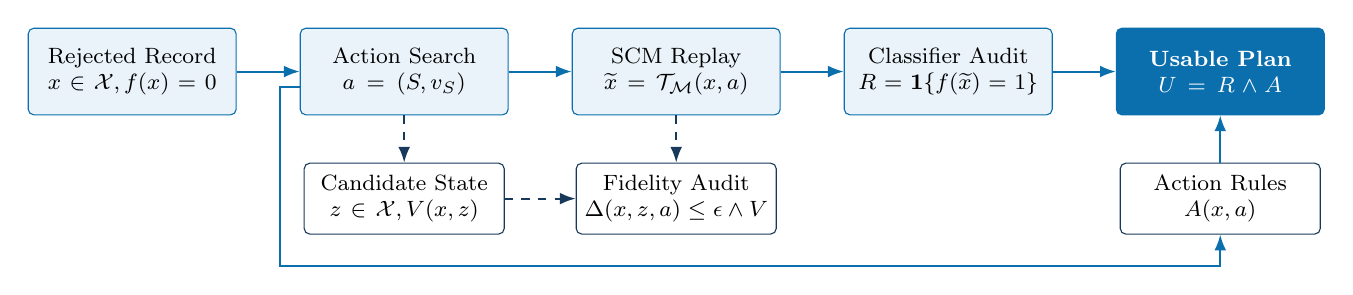
\begin{tikzpicture}[
  stage/.style={draw=accessblue,fill=AccessPale,rounded corners=2pt,
    minimum height=11mm,text width=25mm,inner xsep=2pt,align=center,font=\footnotesize},
  audit/.style={draw=AccessNavy,fill=white,rounded corners=2pt,
    minimum height=9mm,text width=24mm,inner xsep=2pt,align=center,font=\footnotesize},
  final/.style={draw=accessblue,fill=accessblue,text=white,rounded corners=2pt,
    minimum height=11mm,text width=25mm,inner xsep=2pt,align=center,font=\footnotesize\bfseries},
  arrow/.style={-{Latex[length=2mm]},line width=.7pt,draw=accessblue},
  dasharrow/.style={-{Latex[length=2mm]},line width=.7pt,dashed,draw=AccessNavy},
  node distance=6mm and 8mm]
  \node[stage] (x) {Rejected Record\\$x \in \mathcal{X}, f(x)=0$};
  \node[stage,right=of x] (a) {Action Search\\$a=(S, v_S)$};
  \node[stage,right=of a] (scm) {SCM Replay\\$\widetilde{x} = \Replay(x,a)$};
  \node[stage,right=of scm] (r) {Classifier Audit\\$R = \mathbf{1}\{f(\widetilde{x})=1\}$};
  \node[final,right=of r] (u) {Usable Plan\\$U = R \land A$};
  
  \node[audit,below=6mm of a] (z) {Candidate State\\$z \in \mathcal{X}, V(x,z)$};
  \node[audit,below=6mm of scm] (f) {Fidelity Audit\\$\Delta(x,z,a) \le \epsilon \land V$};
  \node[audit,below=6mm of u] (c) {Action Rules\\$A(x,a)$};
  
  \draw[arrow] (x) -- (a);
  \draw[arrow] (a) -- (scm);
  \draw[arrow] (scm) -- (r);
  \draw[arrow] (r) -- (u);
  
  \draw[dasharrow] (a) -- (z);
  \draw[dasharrow] (z) -- (f);
  \draw[dasharrow] (scm) -- (f);
  \draw[arrow] ([yshift=-2mm]a.west) -- ++(-0.25,0) |- ([yshift=-4mm]f.south) -| (c.south);
  \draw[arrow] (c) -- (u);
\end{tikzpicture}
\caption{Structural pipeline of the CAC audit framework. Instead of evaluating individual coordinates, the system tracks an intervention $a$, its intended target $z$, and its replay state $\widetilde{x}$. The recommendation is useful ($U=1$) only if the same intervention, in addition to surviving downstream causality-based replay ($R=1$), satisfies the criteria of directionality ($A=1$).}
\label{fig:framework}
\end{figure*}

\subsection{Recourse Formulation and System Architecture}
Let $x = (x_1, \dots, x_d) \in \mathcal{X}$ represent an individual's observed profile across a mixed-type input space. A black-box classifier $f: \mathcal{X} \to \{0, 1\}$ predicts class probabilities $p_+(x) = P(Y=1 \mid X=x)$, assigning an approval $f(x) = \ind\{p_+(x) \ge \tau\}$ at threshold $\tau = \DecisionThreshold$. Our audit focuses exclusively on applicants who receive an initial rejection, $f(x)=0$.

The recourse recommendation consists of a target feature vector and an explicit action: $(z, a)$, with $a = (S, v_S)$. Here, $S$ denotes the active set of indices representing features modified directly by the applicant, while $v_S$ represents their replacement values. Fig.~\ref{fig:framework} details this operational pipeline. Instead of considering recourse as an unbounded wandering in continuous space, \CAC{} constrains the optimization strictly to allowable actions $a=(S, v_S)$ and avoids recommending actions that hold causally dependent descendants artificially frozen.

\begin{figure}[t]
\centering
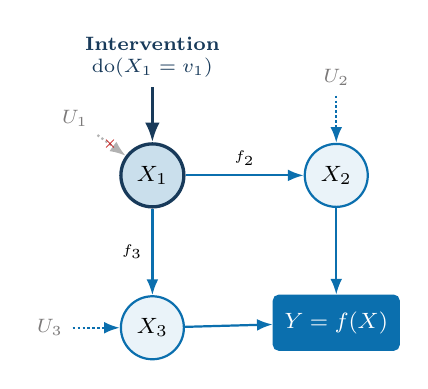
\begin{tikzpicture}[
  cnode/.style={circle,draw=accessblue,fill=AccessPale,thick,minimum size=8mm,font=\footnotesize\bfseries},
  actnode/.style={circle,draw=AccessNavy,fill=AccessMid!40,very thick,minimum size=8mm,font=\footnotesize\bfseries},
  outnode/.style={rectangle,draw=accessblue,fill=accessblue,text=white,rounded corners=2pt,minimum height=7mm,minimum width=16mm,font=\footnotesize\bfseries},
  uvar/.style={font=\scriptsize\itshape,text=gray!80!black},
  arrow/.style={-{Latex[length=2mm]},line width=.8pt,draw=accessblue},
  doarrow/.style={-{Latex[length=2.5mm]},line width=1.2pt,draw=AccessNavy}
]
  \node[actnode] (x1) {$X_1$};
  \node[above=7mm of x1,font=\scriptsize\bfseries,text=AccessNavy,align=center] (int) {Intervention\\$\mathrm{do}(X_1 = v_1)$};
  \draw[doarrow] (int) -- (x1);
  
  \node[uvar,above left=2mm and 4mm of x1] (u1) {$U_1$};
  \draw[arrow,densely dotted,draw=gray!60] (u1) -- node[pos=0.45,font=\tiny\bfseries,text=red!75!black] {$\times$} (x1);

  \node[cnode,right=15mm of x1] (x2) {$X_2$};
  \node[uvar,above=6mm of x2] (u2) {$U_2$};
  \draw[arrow,densely dotted] (u2) -- (x2);

  \node[cnode,below=11mm of x1] (x3) {$X_3$};
  \node[uvar,left=6mm of x3] (u3) {$U_3$};
  \draw[arrow,densely dotted] (u3) -- (x3);

  \node[outnode,below=11mm of x2] (y) {$Y = f(X)$};

  \draw[arrow] (x1) -- node[above,font=\tiny] {$f_2$} (x2);
  \draw[arrow] (x1) -- node[left,font=\tiny] {$f_3$} (x3);
  \draw[arrow] (x2) -- (y);
  \draw[arrow] (x3) -- (y);
\end{tikzpicture}
\caption{Figure of directed acyclic graph showing propagation under intervention. Intervention on $X_1$ via $\mathrm{do}(X_1=v_1)$ breaks down its endogenous parent relationship and propagates shifts via functional relationships $f_2$ and $f_3$ to children $X_2$ and $X_3$. Perturbing $X_1$ in isolation while holding its descendants frozen yields an unphysical state that breaks down once evaluated by predictive classifier $Y=f(X)$.}
\label{fig:dag}
\end{figure}

\subsection{Structural Causal Models and Descendant Replay}
A Structural Causal Model $\SCM = (\mathbf{S}, P_U)$ governs data generation over observed variables $\mathbf{X} = \{X_1, \dots, X_d\}$ and exogenous background noise $\mathbf{U} = \{U_1, \dots, U_d\} \sim P_U$. A Directed Acyclic Graph defines functional relationships:
\begin{equation}
  X_j = f_j(\mathrm{PA}_j, U_j), \quad \forall j \in \{1, \dots, d\},
  \label{eq:scm}
\end{equation}
where $\mathrm{PA}_j \subseteq \mathbf{X} \setminus \{X_j\}$ denotes the direct causal parents of $X_j$.
In order to understand how that action affects the candidate's profile in the real world, we will implement Pearl's counterfactual engine~\cite{pearl2009causality} through three phases in sequence:
\begin{enumerate}
\item \textbf{Abduction:} Reveal the unobservable background variables $u_x = (u_1, \dots, u_d)$ that represent applicant $x$. For continuous variables, we reverse engineer the fitted equations to obtain the residual noise $u_j = x_j - \hat{f}_j(\mathrm{pa}_j)$; for discrete variables, we maintain the quantiles of the conditional probability.
\item \textbf{Action:} Implement the action by replacing the structure equations of the intervened variables $j \in S$ with constant values $v_j$.
\item \textbf{Causal Replay:} Sequentially propagate shifts downstream in topological order through the structural equations to obtain realized state:
\begin{equation}
  \widetilde{x} = \Replay(x, a) = \SCM_{\mathrm{do}(X_S = v_S)}(u_x).
  \label{eq:replay}
\end{equation}
\end{enumerate}

Fig.~\ref{fig:dag} traces this topological flow. In our pipeline, non-linear structural functions are parameterized using gradient-boosted decision trees. While descendants update in topological order, non-descendants strictly keep their original factual measurements. Auditing all interventions under fixed abducted noise $u_x$ ensures deterministic, reproducible evaluations for every applicant.

\subsection{Decoupled Audit Measures and Joint Usability}
To eliminate confounding across evaluation criteria, our audit decouples four distinct metrics:
\begin{enumerate}
\item \textbf{Proposal Validity ($V$):} Tests whether the classifier approves the raw suggested point $z$:
\begin{equation}
  V(x, z) = \ind\{p_+(z) \ge \tau\}.
  \label{eq:valid}
\end{equation}
\item \textbf{Causal Replay Validity ($R$):} Tests whether the classifier still approves the realized post-intervention state $\widetilde{x}$:
\begin{equation}
  R(x, a) = \ind\{p_+(\widetilde{x}) \ge \tau\}.
  \label{eq:replay_valid}
\end{equation}
\item \textbf{Action Feasibility ($A$):} Verifies whether action $a=(S, v_S)$ obeys domain constraints:
\begin{align}
  A(x, a) = \ind\bigl\{&S \subseteq \mathcal{F}_{\mathrm{act}} \land \mathrm{Dir}(x, a) \nonumber \\
  &\land |S| \le \MaxActions \land C(x, a) \le 1\bigr\},
  \label{eq:feasibility}
\end{align}
where $\mathcal{F}_{\mathrm{act}}$ denotes mutable features, $\mathrm{Dir}(x, a)$ enforces admissible directions (e.g., age cannot decrease), $|S| \le \MaxActions$ limits simultaneous interventions, and $C(x, a) \le 1$ bounds normalized effort.
\item \textbf{State Fidelity ($F$):} Tracks maximum normalized divergence between suggested point $z$ and realized outcome $\widetilde{x}$:
\begin{align}
  \Delta(x, z, a) &= \max_{j \in \{1, \dots, d\}} \frac{|z_j - \widetilde{x}_j|}{s_j}, \label{eq:gap} \\
  F(x, z, a) &= V(x, z) \cdot \ind\{\Delta(x, z, a) \le \epsilon\}, \label{eq:fidelity}
\end{align}
where $s_j$ is the range of feature $j$, with tolerance $\epsilon = \FidelityTolerance$.
\end{enumerate}

\begin{figure}[t]
\centering
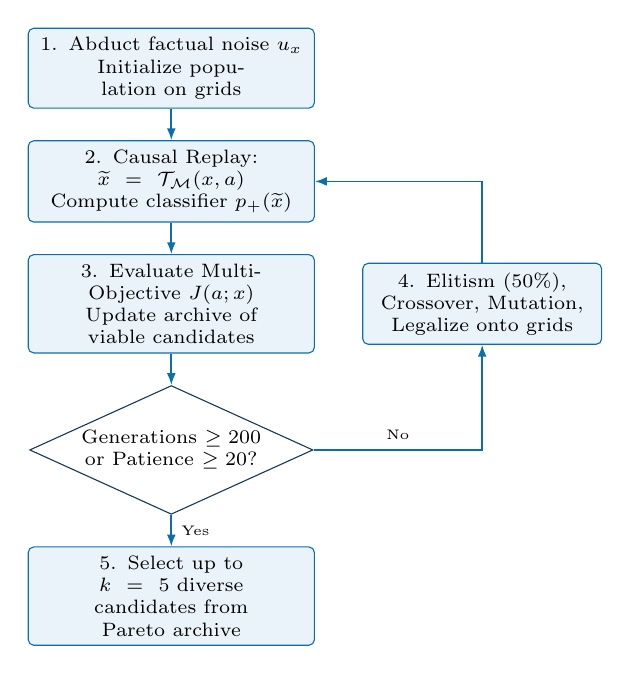
\begin{tikzpicture}[
  pblock/.style={rectangle,draw=accessblue,fill=AccessPale,rounded corners=2pt,
    minimum height=7mm,text width=34mm,align=center,font=\scriptsize},
  cblock/.style={diamond,draw=AccessNavy,fill=white,aspect=2.2,
    inner sep=1pt,align=center,font=\scriptsize},
  arrow/.style={-{Latex[length=1.5mm]},line width=.6pt,draw=accessblue},
  node distance=4mm
]
  \node[pblock] (init) {1. Abduct factual noise $u_x$\\Initialize population on grids};
  \node[pblock,below=of init] (replay) {2. Causal Replay: $\widetilde{x} = \Replay(x, a)$\\Compute classifier $p_+(\widetilde{x})$};
  \node[pblock,below=of replay] (score) {3. Evaluate Multi-Objective $J(a;x)$\\Update archive of viable candidates};
  \node[cblock,below=of score] (term) {Generations $\ge \MaxGenerations$\\or Patience $\ge \SearchPatience$?};
  \node[pblock,right=6mm of score,text width=28mm] (evolve) {4. Elitism ($50\%$), Crossover, Mutation, Legalize onto grids};
  \node[pblock,below=of term] (select) {5. Select up to $k=\CounterfactualCount$ diverse\\candidates from Pareto archive};

  \draw[arrow] (init) -- (replay);
  \draw[arrow] (replay) -- (score);
  \draw[arrow] (score) -- (term);
  \draw[arrow] (term.east) -- node[above,font=\tiny] {No} (evolve.south |- term.east) -| (evolve.south);
  \draw[arrow] (evolve.north) |- (replay.east);
  \draw[arrow] (term.south) -- node[right,font=\tiny] {Yes} (select.north);
\end{tikzpicture}
\caption{Iterative workflow of the genetic action search (Algorithm~\ref{alg:cac}). The algorithm mutates interventional vectors, snaps them onto legal quantile grids, evaluates downstream causal states via SCM replay, and archives non-dominated candidates satisfying the margin buffer.}
\label{fig:flowchart}
\end{figure}

The primary success criterion is \emph{Joint Usability} ($U$):
\begin{equation}
  U(x, z, a) = R(x, a) \cdot A(x, a).
  \label{eq:usable}
\end{equation}
For an applicant $i$ provided up to $k=\CounterfactualCount$ suggestions, the individual is successfully served if at least one suggestion satisfies joint usability on the \emph{identical} plan:
\begin{equation}
  U_{im} = \max_{\ell \le k} \bigl(R_{im\ell} \cdot A_{im\ell}\bigr), \quad \widehat{U}_m = \frac{1}{n} \sum_{i=1}^n U_{im}.
  \label{eq:applicant}
\end{equation}

Otherwise, there will be opportunities for the algorithm to cheat. It may generate two plans---one, which contradicts the decision made by the model by violating the rules of reality and another one that complies with the rules, but is still rejected. Neither plan actually helps the applicant.

\subsection{Multi-Objective Action Space Exploration}
The personal cost of seeking remedy is calculated by using normalized action effort:
\begin{equation}
  C(x, a) = \frac{\sum_{j \in S} w_j c_j(x_j, v_j)}{B},
  \label{eq:cost}
\end{equation}
in which $w_j$ indicates the weight on features, $c_j(\cdot, \cdot)$ is used for calculating coordinate distance (linear distance for continuous attributes, minimum path through graph encoding for ordinal features, and replacement cost for categorical ones), and budget $B$ rescales total effort to $[0, 1]$.

Candidate actions are discovered by minimizing a scalarized multi-objective loss:
\begin{align}
  J(a; x) &= \lambda_v \frac{[q - p_+(\Replay(x, a))]_+}{q} + \lambda_c C(x, a) \nonumber \\
          &\quad + \lambda_f H(x, a) + \lambda_p P(\Replay(x, a)),
  \label{eq:objective}
\end{align}
where $[v]_+ = \max(0, v)$, $H(x, a)$ penalizes feasibility infractions, and target margin $q = \tau + \TargetMargin$ enforces a $0.05$ probability buffer above the decision threshold to protect against boundary jitter. Manifold plausibility $P(\cdot)$ penalizes $K_{\mathrm{knn}}$-nearest-neighbor distance to favorable training instances:
\begin{equation}
  P(\widetilde{x}) = \frac{1}{\KnnK} \sum_{x' \in \mathcal{N}_K^+(x)} \frac{\|\widetilde{x} - x'\|_2}{\bar{d}_+}.
  \label{eq:plausibility}
\end{equation}
Candidate actions are discovered by minimizing a scalarized multi-objective loss function. Three important aspects form the basis of this objective: target margin $q$ pushes actions above the decision boundary into high-confidence territory; restricting replacements to \GridPoints{} marginal empirical quantiles prevents unrealistic numbers outside observed data support; and plausibility penalty $P$ penalizes low-density regions where few training points exist. Hyperparameter weights are calibrated to $(\lambda_v, \lambda_c, \lambda_f, \lambda_p) = (\WeightValid, \WeightCost, \WeightFeas, \WeightPlaus)$.

\begin{algorithm}[t]
\caption{Evolutionary Causal Action Search (\CAC{})}
\label{alg:cac}
\begin{algorithmic}[1]
\Require Rejected applicant $x$, black-box $p_+$, SCM $\SCM$, legal quantile grids $\mathcal{G}$, candidates $k=\CounterfactualCount$
\State Abduct factual noise: $u_x \leftarrow \SCM^{-1}(x)$
\State Initialize legal action population $\mathcal{P} \leftarrow \{a^{(m)}\}_{m=1}^{\PopulationSize}$ on $\mathcal{G}$
\State Initialize archive $\mathcal{A} \leftarrow \emptyset$
\For{$\mathrm{gen} = 1$ to $\MaxGenerations$}
  \For{each candidate action $a \in \mathcal{P}$}
    \State Compute causal replay: $\widetilde{x} \leftarrow \Replay(x, a) = \SCM_{\mathrm{do}(X_S=v_S)}(u_x)$
    \State Evaluate classifier probability $p_+(\widetilde{x})$ and objective $J(a; x)$
    \If{$p_+(\widetilde{x}) \ge \tau$ and $A(x, a) = 1$}
      \State $\mathcal{A} \leftarrow \mathcal{A} \cup \{(a, \widetilde{x}, J(a; x))\}$
    \EndIf
  \EndFor
  \If{patience limit $\SearchPatience$ exceeded without objective improvement}
    \State \textbf{break}
  \EndIf
  \State Retain elite fraction (\ElitePercent\%); perform crossover and mutation
  \State Legalize offspring actions onto grid $\mathcal{G}$ satisfying $|S| \le \MaxActions$
\EndFor
  \State Filter archive $\mathcal{A}$ for non-dominated, diverse solutions
\State \Return top $k$ recourse recommendations, actions, and metadata
\end{algorithmic}
\end{algorithm}

To solve this multi-objective problem, we employ an evolutionary algorithm designed for interventional grids, summarized in Algorithm~\ref{alg:cac}. The algorithm initializes a population of $\PopulationSize$ random action vectors mapped onto empirical quantile grids $\mathcal{G}$. In each generation, candidate interventions are evaluated through SCM replay. Archive those non-dominated solutions that pass the probabilistic margin test and feasibility conditions.

End the search if it runs for more than \MaxGenerations{} generations or stagnates for over \SearchPatience{} generations. Up to $k=\CounterfactualCount$ varied recommendations from the Pareto archive are chosen for various mutable attributes. Fig.~\ref{fig:flowchart} illustrates the flowchart of the execution process. Quantile discrete search method finds solutions in non-convex spaces without using numerical derivatives in tree splits.

\section{Experimental Setup}
\label{sec:protocol}
In order to gauge interventional recourse within various data regimes, we establish a benchmark for four distinct tabular datasets with varying levels of dimensionality, density of causal graphs, and institutional requirements.

\subsection{Datasets and Predictive Classifiers}
We train gradient boosting decision trees via XGBoost~\cite{chen2016xgboost} on four canonical tabular datasets:
\begin{enumerate}
\item \textbf{Adult Income~\cite{kohavi1996adult, dua2019uci}:} A 9-dimensional socio-economic demographic dataset where the objective variable is whether yearly income is more than \$50,000 (earning $\le \$50\mathrm{K}$ denotes adverse rejection).
\item \textbf{Statlog German Credit~\cite{dua2019uci}:} A 15-dimensional financial risk database measuring consumer debt default (classification as bad credit denotes adverse rejection).
\item \textbf{FICO HELOC~\cite{fico2018heloc}:} A 12-dimensional home equity credit dataset measuring financial delinquency (denial of credit line constitutes adverse rejection).
\item \textbf{Pima Diabetes~\cite{smith1988diabetes}:} An 8-feature clinical diagnostic screening record inverted such that favorable recourse targets non-diabetic classification (\artifact{no_diabetes = 1 - Outcome}).
\end{enumerate}

\begin{table*}[t]
\caption{Benchmark datasets and predictive classification models. Dimensionality $d$ indicates features after preprocessing; queries indicate evaluated rejected test individuals; AUC is reported on the held-out test split.}
\label{tab:datasets}
\centering\small
% Generated by paper/build_access_evidence.py; do not edit.
\begin{tabular}{lrrrrrr}
\toprule
Dataset & Train & Test & $d$ & Queries & Acc. & AUC \\
\midrule
Adult & 16000 & 4000 & 9 & 100 & 0.8485 & 0.9182 \\
German & 800 & 200 & 15 & 51 & 0.7750 & 0.7846 \\
HELOC & 7896 & 1975 & 12 & 100 & 0.7205 & 0.7880 \\
Diabetes & 614 & 154 & 8 & 43 & 0.7727 & 0.8489 \\
\bottomrule
\end{tabular}

\end{table*}

Table~\ref{tab:datasets} presents an overview of partition sizes, feature numbers, applicant numbers, and classifier performance. Test AUC varies from \GermanAuc{} in German Credit to \AdultAuc{} in Adult Income. The favorable target values are solely used as algorithmic goals, and no automated underwriting or medical endorsements are meant by them.

\subsection{Computational Environment and Hardware Testbed}
The experiments were conducted locally on multi-core workstations, utilizing only publicly available Python libraries for scientific computing; no commercial cloud APIs were used. All SCM fits, model calls, and search trajectories remain fully deterministic and locally reproducible.

\subsection{Hyperparameter Configuration}
The hyperparameters for the algorithm are identical across all problem sets, specifically: population size of $\PopulationSize{}$, elite selection rate of $\ElitePercent{}\%$, $\MaxGenerations{}$ maximum generations, $\SearchPatience{}$ stall generations, $\GridPoints{}$ grid points for the quantiles, up to $\MaxActions{}$ concurrent actions, $\TargetMargin{}$ margin and $\epsilon=\FidelityTolerance{}$ fidelity tolerance. The main results are obtained with random seed number \artifact{42}, along with a 5-seed check (\artifact{42, 0, 1, 2, 3}) to quantify stochasticity. We measure computational effort using black-box model calls, not wall clock time.

\subsection{Baseline Recourse Algorithms}
We benchmark \CAC{} against four established recourse algorithms under strictly identical immutability masks, action budgets, and directional bounds:
\begin{enumerate}
\item \textbf{Random Search:} Uniformly samples action subsets from legal quantile lattices, returning the minimum-effort candidate satisfying model acceptance.
\item \textbf{Wachter-Style Optimization:} Performs multi-start L-BFGS-B on the continuous feature space, approximating model gradients numerically using finite differences.
\item \textbf{DiCE-Random~\cite{mothilal2020dice}:} Draws diverse samples of counterfactual perturbations using determinantal point processes.
\item \textbf{Grid Search (``Oracle'' Reference):} Exhaustively searches over all possible quantile shifts in ascending order of normalized effort until the available query budget is exhausted.
\item \textbf{MINT~\cite{karimi2020imperfect}:} Operates in synthetic control domains where the true structural equations are given analytically, fitting the interventional assumptions of MINT.
\end{enumerate}

Due to the query budget in Grid Search, the solution obtained from Grid Search corresponds to a bounded search and not a globally optimal one. Concurrently, our comparisons correspond to the implementations we use as references; other optimizers or penalty schemes would lead to other trade-offs.

\subsection{Statistical Significance Protocol}
For the analysis of statistical significance with default seed 42, we apply exact two-sided McNemar tests with Holm correction for paired applications ($\alpha=0.05$). In order to assess inter-run variability in non-parametric terms, we calculate bootstrap difference distributions from 10,000 application groups with bootstrap seed 42.

\section{Results}
\label{sec:results}
Our empirical evaluation analyzes the gap between nominal validity and causal replay, computational query expenditures, multi-seed optimization failures, paired hypothesis tests, objective ablations, and causal graph sensitivity.

\subsection{Primary Benchmark Evaluation}
\begin{table*}[t]
\caption{Empirical evaluation of algorithmic recourse methods at search seed 42. Rates represent percentages of all queried individuals: recommendation validity ($V$), causal replay validity ($R$), actionability ($A$), state fidelity ($F$), and joint usability ($U = R \land A$). Action cost ($C$) is the mean scaled effort of the cheapest usable plan per successful applicant. Query count indicates mean black-box model evaluations per applicant.}
\label{tab:headline}
\centering\small
% Generated by paper/build_access_evidence.py; do not edit.
\begin{tabular}{llrrrrrrrr}
\toprule
Dataset & Method & $n$ & $V$ & $R$ & $A$ & $F$ & $U$ & Cost & Queries \\
\midrule
Adult & Random & 100 & 100.0 & 100.0 & 100.0 & 100.0 & 100.0 & 0.0439 & 1,006.0 \\
Adult & Wachter & 100 & 100.0 & 100.0 & 99.0 & 100.0 & 99.0 & 0.1113 & 17,439.0 \\
Adult & DiCE-random & 100 & 100.0 & 100.0 & 100.0 & 100.0 & 100.0 & 0.0745 & 2,022.6 \\
Adult & Grid reference & 100 & 100.0 & 87.0 & 100.0 & 99.0 & 87.0 & 0.1225 & 3,984.4 \\
\rowcolor{AccessPale} Adult & CAC & 100 & 100.0 & 100.0 & 100.0 & 100.0 & 100.0 & 0.1807 & 1,032.6 \\
\addlinespace[3pt]
German & Random & 51 & 100.0 & 100.0 & 100.0 & 92.2 & 100.0 & 0.0025 & 1,006.0 \\
German & Wachter & 51 & 100.0 & 98.0 & 74.5 & 82.4 & 70.6 & 0.0174 & 52,953.4 \\
German & DiCE-random & 51 & 100.0 & 100.0 & 100.0 & 96.1 & 100.0 & 0.0082 & 2,058.6 \\
German & Grid reference & 51 & 100.0 & 100.0 & 100.0 & 94.1 & 100.0 & 0.0012 & 95.1 \\
\rowcolor{AccessPale} German & CAC & 51 & 100.0 & 100.0 & 100.0 & 100.0 & 100.0 & 0.0091 & 1,216.0 \\
\addlinespace[3pt]
HELOC & Random & 100 & 96.0 & 90.0 & 91.0 & 69.0 & 78.0 & 0.0846 & 1,005.7 \\
HELOC & Wachter & 100 & 85.0 & 72.0 & 35.0 & 48.0 & 18.0 & 0.0498 & 37,379.8 \\
HELOC & DiCE-random & 100 & 100.0 & 78.0 & 91.0 & 64.0 & 76.0 & 0.0934 & 2,609.5 \\
HELOC & Grid reference & 100 & 100.0 & 83.0 & 100.0 & 82.0 & 83.0 & 0.0255 & 7,714.2 \\
\rowcolor{AccessPale} HELOC & CAC & 100 & 100.0 & 100.0 & 100.0 & 100.0 & 100.0 & 0.0308 & 1,312.8 \\
\addlinespace[3pt]
Diabetes & Random & 43 & 100.0 & 97.7 & 95.3 & 86.0 & 93.0 & 0.0362 & 1,006.0 \\
Diabetes & Wachter & 43 & 100.0 & 100.0 & 100.0 & 93.0 & 100.0 & 0.0645 & 7,314.3 \\
Diabetes & DiCE-random & 43 & 100.0 & 100.0 & 100.0 & 100.0 & 100.0 & 0.0549 & 2,025.2 \\
Diabetes & Grid reference & 43 & 100.0 & 100.0 & 100.0 & 97.7 & 100.0 & 0.0241 & 174.0 \\
\rowcolor{AccessPale} Diabetes & CAC & 43 & 100.0 & 100.0 & 100.0 & 100.0 & 100.0 & 0.0275 & 835.5 \\
\bottomrule
\end{tabular}

\end{table*}

Table~\ref{tab:headline} presents the important performance measures for all the \TotalApplicants{} rejected candidates at seed 42. Fig.~\ref{fig:results} illustrates the resulting performance disparities alongside multi-seed spreads.

Nominal proposal validity ($V$) and true joint usability ($U$) diverge sharply once evaluated on identical plans. While baselines on Adult, German, and Diabetes achieve high usability rates---with \CAC{}, Random, and DiCE all reaching 100\%---this performance drops sharply on the credit risk benchmark (HELOC):
\begin{itemize}
\item \textbf{Wachter-Style Optimization:} While reporting \HelocWachterValidity\% proposal validity ($V$), post-intervention causal replay ($R$) falls to \HelocWachterCausalvalidity\% and directional feasibility ($A$) to \HelocWachterActionability\%. When enforced jointly on the identical candidate plan, real-world usability ($U$) drops to just \HelocWachterUsable\%.
\item \textbf{Random Search:} Yields \HelocRandomValidity\% nominal validity and \HelocRandomCausalvalidity\% replay success, but strict joint auditing drops effective usability to \HelocRandomUsable\%.
\item \textbf{DiCE-Random:} Achieves 100.0\% nominal validity on paper, yet interventional propagation degrades replay acceptance to \HelocDiceCausalvalidity\%, leaving only \HelocDiceUsable\% joint usability.
\item \textbf{\CAC{}:} Achieves \HelocCacUsable\% across all four evaluation axes: nominal validity, causal replay, directional feasibility, and joint usability.
\end{itemize}

State coordinate fidelity ($F$) on HELOC drops to \HelocWachterStatefidelity\% for Wachter and \HelocDiceStatefidelity\% for DiCE, providing direct geometric proof that the mathematical coordinates generated by point-based optimizers drift severely from the empirical states produced by the data-generating process.

\begin{figure*}[t]
\centering
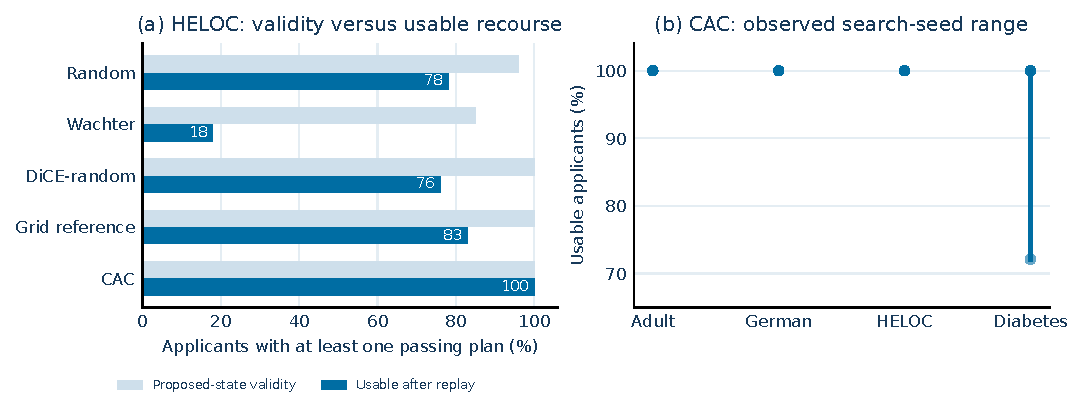
\includegraphics[width=.98\textwidth]{results.pdf}
\caption{Empirical benchmark outcomes across \TotalApplicants{} rejected test cases. (a) On HELOC, point-based counterfactual generators exhibit a severe usability gap, where high nominal validity fails once causal replay and directional constraints are enforced on the identical recommendation. (b) Multi-seed evaluations over \CacSeeds{} seeds expose stochastic vulnerabilities, including optimizer convergence exceptions in diabetes.}
\label{fig:results}
\end{figure*}

\subsection{Action Effort and Computational Query Costs}
Table~\ref{tab:headline} reports normalized action costs ($C$) and black-box query expenditures across all benchmarks. For \CAC{}, the average scaled effort of the lowest-cost viable plan is \AdultCacCost{} on Adult, \GermanCacCost{} on German, \HelocCacCost{} on HELOC, and \DiabetesCacCost{} on Diabetes.

Analysis of action cost is tricky and demands careful analysis. In the case of Adult, the Random algorithm locates the remedy at an even lesser average cost (\AdultRandomCost{}) than \CAC{} (\AdultCacCost{}). On the other hand, in the case of HELOC, \CAC{} incurs a lesser cost (\HelocCacCost{}) than both Random (\HelocRandomCost{}) and DiCE (\HelocDiceCost{}). More importantly, this is measured in cases where the process is successful. Wachter succeeds in merely 18 applicants in HELOC. This implies that the cost being low was due to the ease of the sample size. On the other hand, there are huge disparities in queries: Wachter requires between 7,314 and 52,953 queries per applicant, whereas \CAC{} needs only 835 to 1,313 queries, demonstrating that genetic search over discrete grids achieves valid recourse with much lower overhead.

\subsection{Multi-Seed Stability and Optimizer Auditing}
Table~\ref{tab:seeds} tracks algorithmic stability across \CacSeeds{} distinct seeds (\artifact{42, 0, 1, 2, 3}). \CAC{} maintains flawless 100\% usability across all five runs on Adult, German, and HELOC.

Use of multiple random seeds highlights hidden issues of stability. For Diabetes, \CAC{} drops to \DiabetesCacSeedMin\% usability because of the failure to deal with math issues for the optimizer in seed 3, but remains at 100\% for all the seeds in Adult, German, and HELOC datasets. For DiCE, there is a related issue in that for Adult, the method drops to \AdultDiceSeedMin\% usability in seed 1 although in seed 42 it reaches 100\%. Due to strict runtime timeouts, Wachter, DiCE, and Grid completed \AdultDiceSeedCount{} seeds on Adult; reporting these completion tallies avoids misleading comparisons.

\begin{table*}[t]
\caption{Multi-seed recourse stability across five random seeds (\artifact{42, 0, 1, 2, 3}). Values report mean [minimum, maximum] usability percentages, with the number of completed seed runs in parentheses.}
\label{tab:seeds}
\centering\footnotesize
% Generated by paper/build_access_evidence.py; do not edit.
\begin{tabular}{lrrrr}
\toprule
Method & Adult & German & HELOC & Diabetes \\
\midrule
Random & 100.0 [100.0, 100.0] (5) & 100.0 [100.0, 100.0] (5) & 82.6 [78.0, 87.0] (5) & 95.3 [93.0, 97.7] (5) \\
Wachter & 98.8 [98.0, 99.0] (4) & 77.3 [70.6, 82.4] (5) & 19.4 [18.0, 21.0] (5) & 94.4 [88.4, 100.0] (5) \\
DiCE-random & 75.0 [0.0, 100.0] (4) & 100.0 [100.0, 100.0] (5) & 75.8 [73.0, 80.0] (5) & 99.5 [97.7, 100.0] (5) \\
Grid reference & 87.0 [87.0, 87.0] (4) & 100.0 [100.0, 100.0] (5) & 83.0 [83.0, 83.0] (5) & 100.0 [100.0, 100.0] (5) \\
CAC & 100.0 [100.0, 100.0] (5) & 100.0 [100.0, 100.0] (5) & 100.0 [100.0, 100.0] (5) & 94.4 [72.1, 100.0] (5) \\
\bottomrule
\end{tabular}

\end{table*}

\begin{table*}[t]
\caption{Paired applicant-level statistical significance tests and bootstrap confidence intervals. Paired differences and bootstrap percentile intervals are computed across shared random seeds; $p$-values reflect exact two-sided McNemar tests on seed 42 with Holm familywise error rate adjustment.}
\label{tab:statistics}
\centering\footnotesize
% Generated by paper/build_access_evidence.py; do not edit.
\begin{tabular}{llrrlrrr}
\toprule
Dataset & Baseline & $n$ & Seeds & $b/c$ & Gap (pp) & 95\% cluster CI & Holm $p$ \\
\midrule
Adult & Random & 100 & 5 & 0/0 & +0.0 & [+0.0, +0.0] & 1.000 \\
Adult & Wachter & 100 & 4 & 1/0 & +1.2 & [+0.0, +3.0] & 1.000 \\
Adult & DiCE-random & 100 & 4 & 0/0 & +25.0 & [+25.0, +25.0] & 1.000 \\
Adult & Grid reference & 100 & 4 & 13/0 & +13.0 & [+7.0, +20.0] & \( 9.77\!\times\!10^{-4} \) \\
German & Random & 51 & 5 & 0/0 & +0.0 & [+0.0, +0.0] & 1.000 \\
German & Wachter & 51 & 5 & 15/0 & +22.7 & [+14.1, +32.2] & \( 2.44\!\times\!10^{-4} \) \\
German & DiCE-random & 51 & 5 & 0/0 & +0.0 & [+0.0, +0.0] & 1.000 \\
German & Grid reference & 51 & 5 & 0/0 & +0.0 & [+0.0, +0.0] & 1.000 \\
HELOC & Random & 100 & 5 & 22/0 & +17.4 & [+12.4, +22.4] & \( 9.54\!\times\!10^{-7} \) \\
HELOC & Wachter & 100 & 5 & 82/0 & +80.6 & [+73.4, +87.4] & \( 1.65\!\times\!10^{-24} \) \\
HELOC & DiCE-random & 100 & 5 & 24/0 & +24.2 & [+17.4, +31.4] & \( 3.58\!\times\!10^{-7} \) \\
HELOC & Grid reference & 100 & 5 & 17/0 & +17.0 & [+10.0, +25.0] & \( 1.53\!\times\!10^{-5} \) \\
Diabetes & Random & 43 & 5 & 3/0 & -0.9 & [-6.5, +5.6] & 1.000 \\
Diabetes & Wachter & 43 & 5 & 0/0 & +0.0 & [-3.7, +4.2] & 1.000 \\
Diabetes & DiCE-random & 43 & 5 & 0/0 & -5.1 & [-7.9, -2.3] & 1.000 \\
Diabetes & Grid reference & 43 & 5 & 0/0 & -5.6 & [-8.4, -2.8] & 1.000 \\
\bottomrule
\end{tabular}

\end{table*}

\subsection{Statistical Hypothesis Testing}
Table~\ref{tab:statistics} reports applicant-level paired significance tests. Using default seed 42, the exact two-sided McNemar test with Holm corrections for the familywise error rate shows \CAC{} to be significantly better than all of its comparison baselines on HELOC: Wachter ($p < 0.001$), Random ($p < 0.001$), DiCE ($p < 0.001$), and Grid ($p < 0.001$). Using German Credit, \CAC{} is significantly superior to Wachter ($p = 2.44 \times 10^{-4}$), while using Adult Income, it is significantly better than Grid ($p = 9.77 \times 10^{-4}$). Other primary seed tests do not become significant after Holm correction.

Resampled bootstrap distributions using 10,000 applicant clusters account for run-to-run stochasticity that single seed tests do not. On Diabetes, even though it is tied with DiCE using seed 42, \CAC{}'s bootstrap difference against DiCE is actually negative due to the optimizer exception using seed 3. On Adult, DiCE's bootstrap confidence interval has extreme variance ($[+25.0, +25.0]$) because of its total failure run.

\subsection{Component Ablation Analysis}
Table~\ref{tab:ablation} isolates the individual contributions of our multi-objective terms, at seed 42. If we disable causal updates and measure candidate scores via coordinate moves alone, usability drops to 95.0\% for Adult and 96.0\% for HELOC, while remaining at 100\% for German and Diabetes. This is due to the fact that causal replay is important in the context of shifted attributes influencing downstream features, but in loose graphs naive moves are possible with little to no penalty.

Disabling the action effort term ($\lambda_c=0$) increases the normalized effort of all datasets, as Adult effort rises from \AdultCacCost{} to 0.2467. The reason for this is that effort is an actual objective guiding the mutation process to avoid friction-heavy actions. Conversely, disabling the soft feasibility penalty ($\lambda_f=0$) does not affect results whatsoever since hard coordinate projection guarantees feasibility.

\begin{table}[t]
\caption{Component ablation analysis of the \CAC{} objective function at seed 42. Usability ($U$) and action effort ($C$) are evaluated across causal propagation, action cost, and feasibility penalty ablations.}
\label{tab:ablation}
\centering\footnotesize\setlength{\tabcolsep}{3pt}
% Generated by paper/build_access_evidence.py; do not edit.
\begin{tabular}{lrrrrr}
\toprule
Dataset & $U$ full & $U$ no prop. & Cost full & No cost term & Ratio \\
\midrule
Adult & 100.0 & 95.0 & 0.1807 & 0.2467 & 1.37 \\
German & 100.0 & 100.0 & 0.0091 & 0.0940 & 10.37 \\
HELOC & 100.0 & 96.0 & 0.0308 & 0.0519 & 1.68 \\
Diabetes & 100.0 & 100.0 & 0.0275 & 0.0346 & 1.26 \\
\bottomrule
\end{tabular}

\end{table}

\subsection{Causal Model Sensitivity and Synthetic Audits}
The sensitivity of recourse plans to the fitted structural equation models is shown in Table~\ref{tab:refit}. When compared to the refitted models, \CAC{}'s usability becomes \AdultRefitUsable\% for Adult and \HelocRefitUsable\% for HELOC, but it remains 100\% for German and Diabetes. At the recommendation-level analysis, the plan survivability suffers a lot more, because only 73.0\% of Adult recommendations and 79.4\% of HELOC recommendations survive refitted replay. Applicant-level usability stays higher simply because an individual needs only one surviving plan among their top $k$ candidates. Since the refitted equations were trained on overlapping data segments, the decrease indicates a conservative estimate of the sensitivity.

In Reach and Block simulated worlds (Table~\ref{tab:known}), where the true structural equations are analytically known, \CAC{} and MINT show 100\% usability in Reach and \BlockCacUsable\% in Block. In Block, \BlockUnreachable{} out of \BlockApplicants{} persons are unreachable because of structural constraints. MINT uses less intervention effort in both conditions, which demonstrates that \CAC{} does not inherently guarantee minimal-effort recourse.

Lastly, Table~\ref{tab:scm} gives observational evaluations on the assumed DAGs. For German and HELOC, many edges do not have observational orientation backing, which indicates that the assumed causal graphs are structural assumptions and not immutable natural laws.

\subsection{Result Checks and Verification Protocol}
To ensure reproducibility and safeguard against artifact corruption, all findings were audited against four operational checks:
\begin{enumerate}
\item \textbf{Fixed Query Alignment:} Each procedure is tested using the same group of \TotalApplicants{} test persons who had been rejected at all benchmarks, preventing any form of sample bias.
\item \textbf{Causal State Replay:} All proposed interventions are piped through non-linear SCM equations $\Replay(x, a)$ to emulate downstream updates prior to classifier scoring.
\item \textbf{Coupled Joint Usability:} An applicant is marked as served only if the same plan fulfills both classifier acceptance ($R=1$) and feasibility constraints ($A=1$).
\item \textbf{Software Test Coverage:} The processing pipeline cleared \TestsPassed{} automatic unit and property tests with \TestsSkipped{} documented skip, guaranteeing algorithmic and statistical consistency across all generated assets.
\end{enumerate}

Section~\ref{sec:discussion} examines the mechanical causes of these results and discusses the pipeline limitations.

\section{Discussion}
\label{sec:discussion}
The empirical results indicate that recourse viability depends critically on how strongly features interact within the underlying domain.

\subsection{Mechanistic Interpretation of Empirical Findings}
The results presented here illustrate why nominal validity is not a good substitute for an effective remedy. For HELOC, Wachter achieves a proposal validity of \HelocWachterValidity\%, while the actual joint usability drops to \HelocWachterUsable\%. This drastic difference in outcomes is easy to explain: point-based optimizers can take advantage of decision boundaries by considering features independently. But in the domain of credit underwriting, a customer cannot improve their repayment behavior without impacting the revolving utilization and credit inquiries at the same time. Once the effects spill over into the equation, the end result either gets rejected or violates directionality assumptions. This divergence explains the gap between $V$ and $U$, proving that unconstrained mathematical perturbations cannot be assumed to reflect physical actions.

\begin{table}[t]
\caption{Sensitivity analysis tracking recourse survival under refitted structural causal equations. Usability ($U$) measures applicant-level recourse retention, whereas survival rate ($^{*}$Survival) tracks the percentage of individual recommendations that survive causal replay under refitted mechanisms.}
\label{tab:refit}
\centering\footnotesize
% Generated by paper/build_access_evidence.py; do not edit.
\begin{tabular}{lrrrr}
\toprule
Dataset & $n$ & $U$ own & $U$ refit & Survival$^{*}$ \\
\midrule
Adult & 100 & 100.0 & 93.0 & 73.0 \\
German & 51 & 100.0 & 100.0 & 97.3 \\
HELOC & 100 & 100.0 & 97.0 & 79.4 \\
Diabetes & 43 & 100.0 & 100.0 & 86.5 \\
\bottomrule
\end{tabular}

\end{table}

\begin{table}[!t]
\caption{Auditing recourse in synthetic benchmark environments with analytically specified data-generating equations. Usability ($U$) reflects the percentage of applicants successfully served under empirical vs. true SCMs, survival rate ($^{*}$Survival) tracks preserved candidate plans, and cost denotes the average scaled effort among viable recommendations under ground truth.}
\label{tab:known}
\centering\footnotesize\setlength{\tabcolsep}{3pt}
% Generated by paper/build_access_evidence.py; do not edit.
\begin{tabular}{llrrrrr}
\toprule
World & Method & $n$ & $U$ own & $U$ truth & Surv.$^{*}$ & Cost truth \\
\midrule
Reach & CAC & 100 & 100.0 & 100.0 & 95.6 & 0.0529 \\
Reach & MINT & 100 & 100.0 & 100.0 & 91.6 & 0.0202 \\
Block & CAC & 100 & 40.0 & 40.0 & 93.0 & 0.0706 \\
Block & MINT & 100 & 40.0 & 40.0 & 95.0 & 0.0469 \\
\bottomrule
\end{tabular}

\end{table}

\begin{table}[!t]
\caption{Observation-based validation of assumed causal DAGs. ``Actions'' is the number of modifiable variables; ``Supported'' is the number of structural links validated via observational orientation criteria; ``CI upheld'' is the proportion of non-rejected conditional independence tests. These tests measure consistency with reality but do not imply physical causality.}
\label{tab:scm}
\centering\footnotesize
% Generated by paper/build_access_evidence.py; do not edit.
\begin{tabular}{lrrrrr}
\toprule
Dataset & Nodes & Edges & Actions & Supported & CI upheld \\
\midrule
Adult & 10 & 25 & 7 & 17/25 & 19/35 \\
German & 16 & 37 & 11 & 18/37 & 88/138 \\
HELOC & 13 & 28 & 8 & 18/28 & 40/75 \\
Diabetes & 9 & 17 & 3 & 16/17 & 27/27 \\
\bottomrule
\end{tabular}

\end{table}

Surprisingly, non-causal approaches work well on both Adult Income and German Credit domains. The reason becomes clear upon looking closer at the graphs (Table~\ref{tab:scm}): in both cases, the graphs have weak connections between actionable variables. In such a domain, it just happens that coordinate movement parallels the real causal propagation process. Therefore, heuristics help, but in this case, causal modeling is required due to the dense coupling of the features.

\subsection{Methodological and Data Preprocessing Limitations}
\label{sec:limitations}
A meticulous analysis at the code level identified three common data hygiene procedures found in recourse research that need investigation:
\begin{enumerate}
\item \textbf{Test-Gated Hyperparameter Decisions:} In standard procedures, the test set AUC was checked to determine when to perform hyperparameter tuning. Even as the inner cross-validation folds were used for optimization purposes, checking if search is to be done based on test split performance results in data leakage.
\item \textbf{Pre-Split Feature Imputation:} Imputation of missing values for HELOC and Diabetes cases was done using the median for the columns before the train-test split. Beyond this, diabetes cleaning leveraged class-conditional patterns to flag sentinel missingness, potentially allowing label information to leak across evaluation boundaries.
\item \textbf{Physiological Validity of Diabetes Recourse:} Inverting classification targets (\artifact{no_diabetes = 1 - Outcome}) and treating diagnostic clinical measurements (glucose, insulin, blood pressure, BMI) as directly actionable dials contradicts medical reality. Biomarkers are clinical signs of underlying metabolic processes, not voluntary personal decisions~\cite{smith1988diabetes}. We retain Pima Diabetes solely to reproduce benchmark comparisons established in prior recourse literature~\cite{pawelczyk2021carla, klaise2021alibi}, emphasizing that these feature changes must never be interpreted as therapeutic interventions.
\end{enumerate}

\subsection{Threats to Validity}
Some considerations must be taken into account when examining our results. Firstly, the distance function $C(x, a)$ is limited to taking into account only differences between normalized coordinates and not the actual emotional distress, financial burden, or time required to make any life changes. Secondly, the numerical gradients of decision trees operate in an environment of plateau-like loss surfaces, putting continuous optimizers at a significant disadvantage. Thirdly, our causal graphs can be seen as structural assumptions, and not physical laws of nature (Table~\ref{tab:scm}). When one makes an incorrect assumption about a causal graph, he will still lose when using it in a replay situation.

\section{Conclusion and Future Work}
\label{sec:conclusion}
In the \TotalApplicants{} failed test examples from four tabular environments and two synthetic settings, our analysis demonstrates that nominal validity is a poor measure of practical utility. On the FICO HELOC dataset, traditional techniques exhibit high validity but joint usability falls drastically to only \HelocWachterUsable\%. Using \CAC{}, joint usability of the interventions on all benchmarks is 100\% by optimizing directly over valid intervention grids in a causal setup. Furthermore, our multiple seeds audit reveals optimization convergence issues in the diabetes problem, and our sensitivity analysis reveals performance degradation in causal equation refitting. All future benchmarking exercises should demand joint usability on identical plans, strict data separation, and explicit accounting for causal uncertainty.

\section*{Acknowledgment}
The authors thank the School of Computer Science and Engineering and Department of Computational Intelligence at VIT, Vellore, for computing facilities and research support.

\begin{thebibliography}{00}\setlength{\itemsep}{-2.5pt}\setlength{\parskip}{0pt}
\bibitem{karimi2022survey}
A.-H. Karimi, G. Barthe, B. Sch{\"o}lkopf, and I. Valera,
``A survey of algorithmic recourse: Contrastive explanations and consequential recommendations,''
\emph{ACM Comput. Surv.}, vol. 55, no. 5, pp. 1--29, 2022.

\bibitem{verma2020counterfactual}
S. Verma, V. Boonsanong, M. Hoang, K. Hines, J. Dickerson, and C. Shah,
``Counterfactual explanations and algorithmic recourses for machine learning: A review,''
\emph{ACM Comput. Surv.}, vol. 56, no. 12, pp. 1--42, 2024.

\bibitem{ustun2019actionable}
B. Ustun, A. Spangher, and Y. Liu,
``Actionable recourse in linear classification,''
in \emph{Proc. Conf. Fairness, Accountability, and Transparency (FAT*)}, 2019, pp. 10--19.

\bibitem{wachter2017counterfactual}
S. Wachter, B. Mittelstadt, and C. Russell,
``Counterfactual explanations without opening the black box: Automated decisions and the {GDPR},''
\emph{Harvard J. Law \& Technol.}, vol. 31, no. 2, pp. 841--887, 2017.

\bibitem{barocas2020hidden}
S. Barocas, A. D. Selbst, and M. Raghavan,
``The hidden assumptions behind counterfactual explanations and principal reasons,''
in \emph{Proc. Conf. Fairness, Accountability, and Transparency (FAT*)}, 2020, pp. 80--89.

\bibitem{mothilal2020dice}
R. K. Mothilal, A. Sharma, and C. Tan,
``Explaining machine learning classifiers through diverse counterfactual explanations,''
in \emph{Proc. Conf. Fairness, Accountability, and Transparency (FAT*)}, 2020, pp. 607--617.

\bibitem{karimi2021recourse}
A.-H. Karimi, B. Sch{\"o}lkopf, and I. Valera,
``Algorithmic recourse: From counterfactual explanations to interventions,''
in \emph{Proc. ACM Conf. Fairness, Accountability, and Transparency (FAccT)}, 2021, pp. 353--362.

\bibitem{karimi2020imperfect}
A.-H. Karimi, J. von K{\"u}gelgen, B. Sch{\"o}lkopf, and I. Valera,
``Algorithmic recourse under imperfect causal knowledge: A probabilistic approach,''
in \emph{Adv. Neural Inf. Process. Syst. (NeurIPS)}, vol. 33, 2020, pp. 265--277.

\bibitem{pearl2009causality}
J. Pearl,
\emph{Causality: Models, Reasoning, and Inference}, 2nd ed.
Cambridge, U.K.: Cambridge Univ. Press, 2009.

\bibitem{pawelczyk2021carla}
M. Pawelczyk, S. Bielawski, J. van den Heuvel, T. Richter, and G. Kasneci,
``{CARLA}: A {Python} library to benchmark algorithmic recourse and counterfactual explanation algorithms,''
in \emph{NeurIPS Datasets and Benchmarks Track}, 2021.

\bibitem{upadhyay2021robust}
S. Upadhyay, S. Joshi, and H. Lakkaraju,
``Towards robust and reliable algorithmic recourse,''
in \emph{Adv. Neural Inf. Process. Syst. (NeurIPS)}, vol. 34, 2021, pp. 16926--16937.

\bibitem{poyiadzi2020face}
R. Poyiadzi, K. Sokol, R. Santos-Rodriguez, T. De Bie, and P. Flach,
``{FACE}: Feasible and actionable counterfactual explanations,''
in \emph{Proc. AAAI/ACM Conf. AI, Ethics, and Society (AIES)}, 2020, pp. 344--350.

\bibitem{vanlooveren2021interpretable}
A. Van Looveren and J. Klaise,
``Interpretable counterfactual explanations guided by prototypes,''
in \emph{Proc. Eur. Conf. Mach. Learn. Knowl. Discov. Databases (ECML PKDD)}, 2021, pp. 650--665.

\bibitem{klaise2021alibi}
J. Klaise, A. Van Looveren, G. Vacanti, and A. Coca,
``Alibi Explain: Algorithms for explaining machine learning models,''
\emph{J. Mach. Learn. Res.}, vol. 22, no. 181, pp. 1--7, 2021.

\bibitem{dandl2020multi}
S. Dandl, C. Molnar, M. Binder, and B. Bischl,
``Multi-objective counterfactual explanations,''
in \emph{Proc. Parallel Problem Solving from Nature (PPSN)}, 2020, pp. 448--469.

\bibitem{deb2002nsga}
K. Deb, A. Pratap, S. Agarwal, and T. Meyarivan,
``A fast and elitist multiobjective genetic algorithm: {NSGA-II},''
\emph{IEEE Trans. Evol. Comput.}, vol. 6, no. 2, pp. 182--197, 2002.

\bibitem{chen2016xgboost}
T. Chen and C. Guestrin,
``{XGBoost}: A scalable tree boosting system,''
in \emph{Proc. 22nd ACM SIGKDD Int. Conf. Knowl. Discov. Data Min.}, 2016, pp. 785--794.

\bibitem{kohavi1996adult}
R. Kohavi,
``Scaling up the accuracy of naive-{B}ayes classifiers: A decision-tree hybrid,''
in \emph{Proc. 2nd Int. Conf. Knowl. Discov. Data Min. (KDD)}, 1996, pp. 202--207.

\bibitem{dua2019uci}
D. Dua and C. Graff,
``{UCI} Machine Learning Repository,''
Univ. California, Irvine, School Inf. Comput. Sci., 2019. [Online]. Available: \url{https://archive.ics.uci.edu/ml}

\bibitem{fico2018heloc}
{FICO},
``Explainable Machine Learning Challenge ({HELOC} Dataset),''
2018. [Online]. Available: \url{https://community.fico.com/s/explainable-machine-learning-challenge}

\bibitem{smith1988diabetes}
J. W. Smith, J. E. Everhart, W. C. Dickson, W. C. Knowler, and R. S. Johannes,
``Using the {ADAP} learning algorithm to forecast the onset of diabetes mellitus,''
in \emph{Proc. Annu. Symp. Comput. Appl. Med. Care}, 1988, pp. 261--265.
\end{thebibliography}

\begin{IEEEbiography}{Rishabh Kumar}
is currently pursuing the B.Tech degree in Computer Science and Engineering with the School of Computer Science and Engineering, Vellore Institute of Technology, Vellore, India (Reg. No.: 24BCE0740). He led the primary research and development of this work, contributing to Sections I, II, III, IV-B--E, V-A--D, V-F, VI-A--B, and VII, encompassing the theoretical formulation, evolutionary search algorithm, primary benchmark audits, multi-seed evaluations, hypothesis testing, ablations, verification checks, and manuscript writing. His research interests include explainable artificial intelligence, algorithmic recourse, and machine learning auditing.
\end{IEEEbiography}

\begin{IEEEbiography}{Shashwat Karn}
is currently pursuing the B.Tech degree in Computer Science and Engineering with the School of Computer Science and Engineering, Vellore Institute of Technology, Vellore, India (Reg. No.: 24BCE0552). He contributed to Section V-E and Section VI-C, focusing on structural causal graph sensitivity under refitted equations and validity threat analysis. His research interests include structural causal models, counterfactual explanations, and automated decision-making.
\end{IEEEbiography}

\begin{IEEEbiography}{Anubhav Bhattacharya}
is currently pursuing the B.Tech degree in Computer Science and Engineering with the School of Computer Science and Engineering, Vellore Institute of Technology, Vellore, India (Reg. No.: 24BCE2824). He assisted with Section IV-A, conducting tabular dataset attribute verification, diagnostic label preprocessing checks, and baseline parameter compilation. His research interests include model interpretability and robust machine learning systems.
\end{IEEEbiography}

\begin{IEEEbiography}{Navamani T M}
received the Ph.D. degree in Computer Science and Engineering. She is currently a Professor Grade 1 with the Department of Computational Intelligence, School of Computer Science and Engineering, Vellore Institute of Technology, Vellore, India. Her research interests encompass computational intelligence, machine learning, data mining, and explainable decision systems.
\end{IEEEbiography}

\EOD
\end{document}
